% 8185: Quant Ellen PS1

\documentclass[12pt]{article}
%\usepackage[T1]{fontenc}
%\usepackage{lipsum}
\renewcommand{\baselinestretch}{1.2} 
\usepackage{graphicx}
\usepackage{hyperref}
\hypersetup{
    colorlinks=true,
    urlcolor=blue,
    citecolor=blue
}
\usepackage[export]{adjustbox}
\usepackage{subcaption}
\usepackage{amsmath}
\usepackage{amsfonts}
\usepackage{geometry}
\geometry{a4paper,
 left=3cm,right=3cm,
 top=1.5cm, bottom=1.5cm}

\usepackage{natbib}
\bibliographystyle{apalike}

%\usepackage{natbib}
%setcitestyle{authoryear,open={(},close={)}}
\graphicspath{ {../figs/} }

\begin{document}
%\thispagestyle{myheadings}
%\markright{Indian Statistical Institute, New Delhi\hfill }

\title{Econ 8185: Quant PS1}
\author{Bipul Verma}
\date{\today}
\maketitle

%\tableofcontents{}
\abstract{The present document calculates the value function, policy functions, of a simple economy with stochastic AR(1) shock to labor productivity. The computation is based made on two different methods- Value Function Iteration, Linear Quadratic Approximation. The LQ problem can be solved either by using iteration on Riccati Equation or directly using Vaughan Method. }

\vspace{8cm}

%\begin{center}
%\includegraphics[scale=0.4]{isi_logo.png}
%\end{center}
%\begin{center}
%\begin{Large}
%INDIAN STATISTICAL INSTITUTE, NEW-DELHI.
%\end{Large}
%\end{center}


\newpage

\section{Model}
We have the following growth model: 
\begin{align*}
	& \max_{\{c_t, x_t, h_t\}} \mathbb{E} \beta^t U(c_t, h_t) \\
	\text{subject to } & c_t + x_t = k_t^\theta((1+\gamma_z)^tz_th_t)^{1-\theta} \\
	& N_{t+1}k_{t+1} = [(1-\delta)k_t + x_t]N_t \\
	& \log z_t = \rho \log z_{t-1} + \epsilon_t, \; \; \epsilon\sim N(0, \epsilon)\\
	& h_t + l_t =1\\
	& N_t = (1+\gamma_n)^t .
\end{align*}

Note that in the above growth model we have population growth given by parameter ($\gamma_n$) as well as productivity growth given by parameter ($\gamma_z$). This means that all the variables will have trend growth at steady state given by $(1+\gamma_z)(1+\gamma_n).$ In order to proceed with solving the model we de-trend the variables. The model with de-trended variables can then be written as shown below.

$$\max_{\{\hat{c}_t, h_t , \hat{k}_{t+1}\}} \sum_t \hat{\beta}^t U(\hat{c}_t, h_t)$$

subject to 

$$\hat{c}_t + \tilde \gamma \hat{k}_{t+1} = \hat{F}(\hat{k}_t, h_t, z_t)$$

$$log(z_{t+1}) = \rho log(z_t) + \epsilon_{t+1}$$ 

where $\hat{x} = \frac{x}{(1+\gamma_z)^t}$ variables denotes the de-trended variables with respect to productivity growth, $\hat{F}(\hat k, h, z) = \hat k^{\theta}(zh)^{1-\theta} + (1-\delta)\hat k$, $U(\hat c, h) = log(\hat c) + \psi log(1-h) $, $\tilde\gamma = (1+\gamma_z)(1+\gamma_n)$ and $\hat{\beta} = \beta(1+\gamma_n)$.

\subsection{Parameters}
The parameter values for $\beta, \delta, \gamma_z, \gamma_n$ are based on Prof. Kehoe's \href{http://users.econ.umn.edu/~tkehoe/classes/calibration.pdf}{Notes} on calibrating the growth models. I have not calibrated the other parameters and tried to assume some values to begin with. The parameter values are:
\begin{align*}
	\beta & = 0.95   & \delta &= 0.05   & \psi &= 1.6 \\
	 \gamma_n & = 0.02 & \gamma_z  &= 0.02 & \theta &= 0.34 \\
	 \rho & = 0.5
\end{align*}


\subsection{Steady State}
The first order conditions along with the resource constraints are sufficient to characterize the steady state for the present economy. These conditions are summarized below.
\begin{flalign*}
	\text{MRS:} & \; \; \; \; \; \; \; \; \; \; \; \frac{-U_h(t)}{U_c(t)} = \hat F_h(t) \\
	\text{Euler:} & \; \; \; \; \; \; \; \; \; \; \; \tilde \gamma U_c(t) = \hat \beta U_c(t+1)\hat F_k(t+1) \\
	\text{Resource:} & \; \; \; \; \; \; \; \; \; \; \; \hat c_t + \tilde \gamma \hat k_{t+1} = \hat F(t)	.\end{flalign*}
The MRS, Euler, and Resource constraints forms a system of 3 equations in 3 variables at the steady state. We solve the system numerically to get the steady state values of $\hat{k}, \hat{h}, \hat{c}$. For the above set of parameter values the steady state of the de-trended variables is as follows: $\hat{k}_{ss} = 1.640111, h_{ss} = 0.3543826, \hat{c}_{ss} = 0.4483689$


\section{Value Function Iteration}

\textbf{Algorithm:}\\

\begin{enumerate}
\setlength\itemsep{0em}
\item Create a 2 dimensional grid of capital $(k)$ and labor supply $(h)$.
\item Use subroutine Tauchen.jl to get an evenly spaced grid of shocks $(z)$ along with the Transition Matrix $(P)$ for the AR(1) process for $log(z)$.
\item Create 2 dimensional empty grids for storing value functions and policy functions. 
\item Create a return function $G(k, k', h, z, V_n) = U(c, h) + \hat{\beta}E_z[V_n(k', z')]$ where $c = F(k, h , z) + (1-\delta)k - (1+\gamma_n)(1+\gamma_z)k'$. The expected value is calculated using the transition matrix obtained above.
\item Create a grid search loop to look for the maximum value and the maximisers, i.e for each $(k, z)$, $V_{n+1}(k, z) = \max_{k', h} G(k, k', h, z, V_n)$;   $k'(k, z) , h(k, z) = argmax_{k', h} G(k, k', h, z, V_n)$.
\item Iterate on the loop until convergence: $||V_{n+1} - V_n|| < tolerance$.
\end{enumerate}

\textbf{Results from VFI}

\begin{figure}[h]
    \centering
    \begin{minipage}{0.45\textwidth}
        \centering
        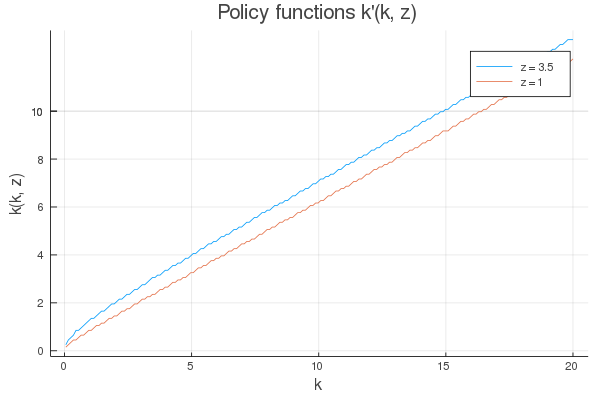
\includegraphics[width=1.2\textwidth]{cap_policy_1_f.png} % first figure itself
        \caption{Capital Policy Function}
    \end{minipage}\hfill
    \begin{minipage}{0.45\textwidth}
        \centering
        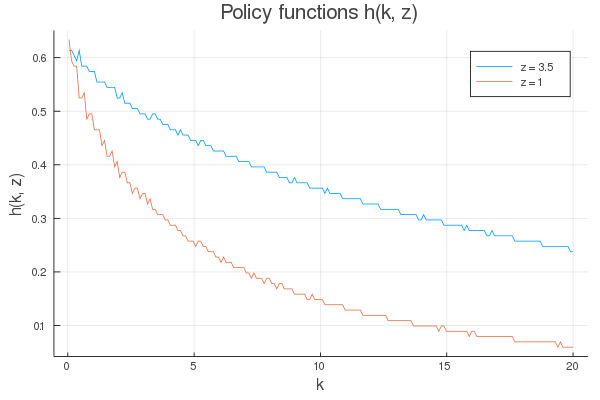
\includegraphics[width=1.2\textwidth]{lab_policy_1_f.png} % second figure itself
        \caption{Labor Policy function}
    \end{minipage}
\end{figure}

\begin{figure}[h]
    \centering
    \begin{minipage}{0.45\textwidth}
        \centering
        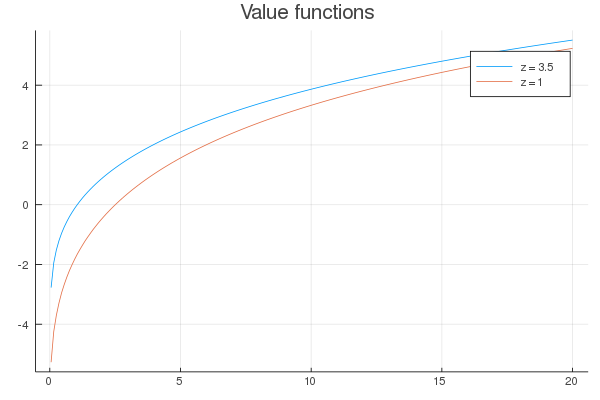
\includegraphics[width=1.2\textwidth]{value_fn_1_f.png} % first figure itself
        \caption{Value Function}
    \end{minipage}\hfill
    \begin{minipage}{0.45\textwidth}
        \centering
        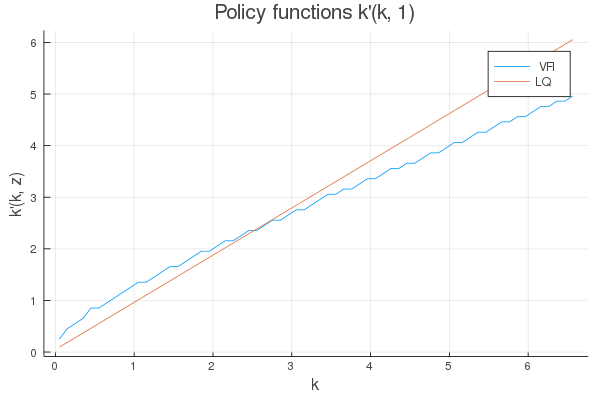
\includegraphics[width=1.2\textwidth]{cap_policy_VFI_LQ.png} % second figure itself
        \caption{Comparision VFI vs LQ}
    \end{minipage}
\end{figure}

\newpage 

\section{LQ Approximation}

% Ref : https://pages.stern.nyu.edu/~dbackus/3386/3386%20notes%205%2004.pdf. 

Linear Quadratic (LQ) are class of problem with quadratic returns being optimized over linear states with linear law of motion. The canonical LQ problem has the following formulation:
\begin{align*}
	\max_{u_t} \sum \beta^t r(X_t, u_t) \\
	\text{s.t. } X_{t+1} = AX_t + Bu_t + C\epsilon_{t+1}.
\end{align*}
A second order Taylor approximation of the return function gives:
\begin{align*}
	r(X, u) & \approx X'QX + u'Ru + 2X'Wu \\
	 & = \begin{bmatrix}
  X \\ u
 \end{bmatrix}' 
  \begin{bmatrix}
 Q & W \\
 W' & R \\
 \end{bmatrix}
 \begin{bmatrix}
 X \\ u
 \end{bmatrix}.
\end{align*}



The quadratic Taylor expansion of the return function is around $(\bar X, \bar u)$ given as:
\begin{multline*}
	r(X, u) \approx r(\bar X, \bar u) + D_X r(\bar X, \bar u)' (X-\bar X) + D_u r(\bar X, \bar u)' (u-\bar u)+ \\
	\frac{1}{2}(X- \bar X)'D^2_{XX}(X-\bar X) +   \frac{1}{2}(u- \bar u)'D^2_{uu}(u-\bar u) + \frac{1}{2}(u- \bar u)'D^2_{uX}(X-\bar X) 
\end{multline*}

The terms in the Taylor expansion can be collected together to obtain $Q, R, W$ as appropriate partitions of the taylor coefficient matrix.
\begin{align*}
	  \begin{bmatrix}
 Q & W \\
 W' & R \\
 \end{bmatrix} = \begin{bmatrix}
 	\bar r & \frac{1}{2}D_X & \frac{1}{2}D_u \\
 	\frac{1}{2}D_X & \frac{1}{2}D_{XX} & \frac{1}{2} D_{uX}\\
 	\frac{1}{2}D_u & \frac{1}{	2}D_{Xu} & \frac{1}{2}D_{uu}
 \end{bmatrix}
\end{align*}

\subsection{(b) (ii) Return function depends on $(k, k', h)$:}
In this case the choice variable $u_t$, and state variable $X_t$ is given as:
\begin{align*}
	u_t = \begin{bmatrix}
		k_{t+1} \\
		h_t
	\end{bmatrix}, \; \; \; X_{t} = \begin{bmatrix}
		1 \\
		k_t\\
		\log z_t
	\end{bmatrix}.
	\end{align*}
Define:

\begin{gather*}
c(k, k', h, z) =  \hat{F}(k, h, z) - (1+\gamma_n)(1+\gamma_z)k'
\end{gather*}
then $$r(X_t, u_t) = U(c(k_t, k_{t+1}, h_t, z_t), h_t).
$$

The coefficients matrices in the law of motion of states $X_{t+1} = A X_t + Bu_t + C\epsilon_{t+1}$, are given below.


$$A= \begin{bmatrix}
1 & 0 & 0\\ 0 & 0 & 0 \\ 0 & 0 & \rho \end{bmatrix}, 
B = \begin{bmatrix} 0 & 0\\ 1 & 0 \\ 0 & 0 \end{bmatrix},
C = \begin{bmatrix} 0 \\ 0 \\  1 \end{bmatrix} .$$


\subsection{(b) (iii) Return function depends on $(k, k')$:}
We use the first order MRS condition along with the resource constraint to solve for $h(k, k', z)$ as implicit solution of the following equation:

 $$\frac{U_h(c(k, k', h, z), h)}{U_c(c(k, k', h, z), h)} = -\hat{F}(k, h, z)$$ 

In the present case $X_t = \begin{bmatrix} 1 \\ k_t \\ log(z_t)\end{bmatrix}, u_t = \begin{bmatrix}k_{t+1} \end{bmatrix}$. The state space representation is as follows:

$$\underbrace{\begin{bmatrix} 1 \\ k_{t+1} \\ log(z_{t+1})\end{bmatrix}}_{X_{t+1}} = \underbrace{\begin{bmatrix}
1 & 0 & 0\\ 0 & 0 & 0 \\ 0 & 0 & \rho \end{bmatrix}}_{A} \underbrace{\begin{bmatrix} 1 \\ k_t \\ log(z_t)\end{bmatrix}}_{X_t} + \underbrace{\begin{bmatrix} 0 \\ 1 \\ 0 \end{bmatrix}}_{B} \underbrace{\begin{bmatrix}k_{t+1} \end{bmatrix}}_{u_t} + \underbrace{\begin{bmatrix} 0 \\ 0 \\ 1 \end{bmatrix}}_{C} \begin{bmatrix} \epsilon_{t+1} \end{bmatrix}  $$ 


\subsection{(c) Vaughan Method}
For Vaughan Method, we closely follow Prof. Ellen's class notes to first construct a matrix $\mathbb{H}$. We then carry out the eigenvalue decomposition of the matrix $\mathbb{H}$. The eigen-vectors are then used to construct the matrices P and F.

\subsection{Results from LQ}
Note that once we have a Linear Quadratic version of our initial problem we can obtain the required matrices by either solving a Riccati equation or using the Vaughan method. We note that both the approaches gives the same answer. The results are outlined below.

\begin{figure}[h]
    \centering
    \begin{minipage}{0.45\textwidth}
        \centering
        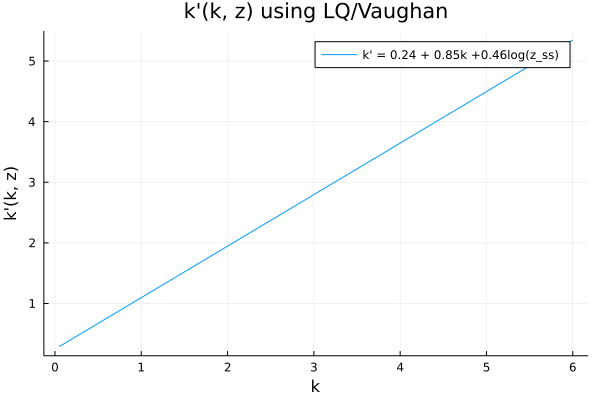
\includegraphics[width=1.2\textwidth]{cap_policy_VLQ.png} % first figure itself
        \caption{Capital Policy Function}
    \end{minipage}\hfill
    \begin{minipage}{0.45\textwidth}
        \centering
        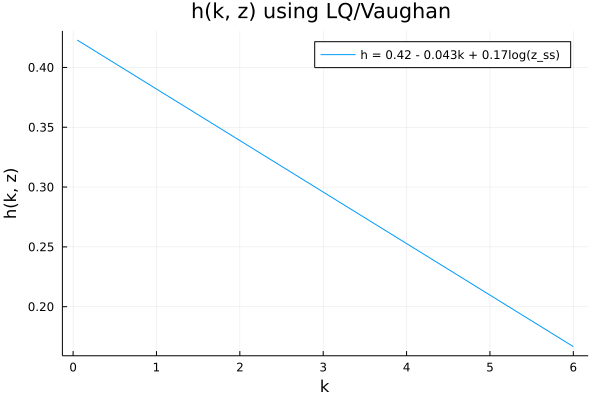
\includegraphics[width=1.2\textwidth]{h_policy_VLQ.png} % second figure itself
        \caption{Labor Policy function}
    \end{minipage}
\end{figure}

We note that the linearized policy function is exactly the same using all of the three formulations mentioned above. The equations for linearized policy functions are reported below:\\
\begin{align*}
k'(k, z) & =  0.245832  +0.850113k   +0.462318 \ln(z)\\
h(k, z) & = 0.425009  - 0.0430618k  +0.171364\ln(z)
\end{align*}
We further note that the LQ approximation can be solved by either solving a Riccati equation or using the Vaughan method. The policy functions derived using the two methods to solve LQ are exactly the same till 6 decimal places.

\section{Time series of output}
Once we have the policy function with using the methods mentioned above, we can simulate the economy to study the time series properties of the output. In the plot below we graph the time series for de-trended per capita output with its steady state level for 200 time periods.
\begin{figure}[h]
    \centering
    \begin{minipage}{0.45\textwidth}
        \centering
        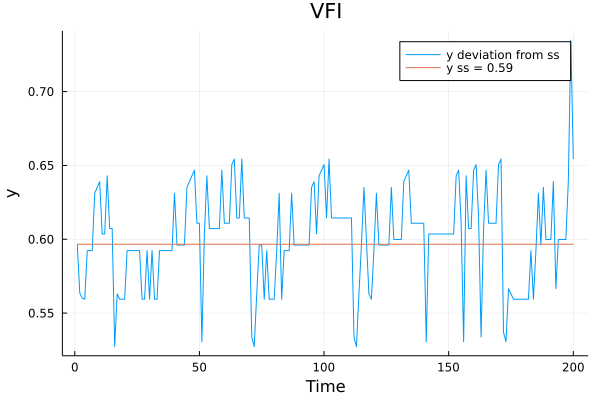
\includegraphics[width=1.2\textwidth]{vfi_y_sim.png} % first figure itself
        \caption{Output deviation VFI}
    \end{minipage}\hfill
    \begin{minipage}{0.45\textwidth}
        \centering
        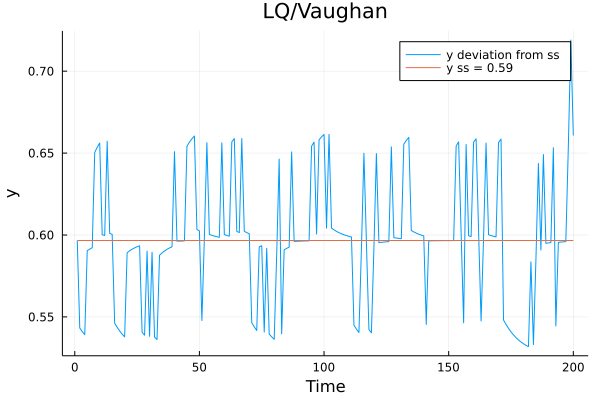
\includegraphics[width=1.2\textwidth]{LQ_y_sim.png} % second figure itself
        \caption{Output deviation LQ/Vaughan}
    \end{minipage}
\end{figure}

We note that de-trended per capita output moves around its steady state value. Since we have approximated the $AR(1)$ shock process using 5 productivity shocks, there are some flat portions in the graph (for some period we draw the same shock). There is slight variation in he result from VFI and LQ/Vaughan due to the fact that VFI is calculated on a limited number of grid points while LQ/Vaughan gives linear policies. However, we note that still the overall pattern of output deviation is close using the two methods.

\section{Properties of Solution }
Note that the code we have written is with non zero values of the parameters $\psi, \delta, \gamma_n, \gamma_z$. Thus, studying the properties of solution by changing parameter values involves changing the initial parameters in the code and re-estimating everything. 
\begin{itemize}
\item When $\psi = 0$ , $h(k, z)$ is a constant for all the cases. This is evident from the VFI, LQ as well as the Vaughan method for such parameter value.
\item When $\delta \neq 1$, the steady state value of capital is higher.
\item When $\gamma_z, \gamma_n =0$, the steady state value of capital is lower.
\end{itemize}




\section{Alternate Utility Function}

The preference are $U(c, h) = \frac{(c(1-h)^{\psi})^{1-\gamma}}{1-\gamma}$  with $\gamma = 5$

\begin{figure}[h]
    \centering
    \begin{minipage}{0.45\textwidth}
        \centering
        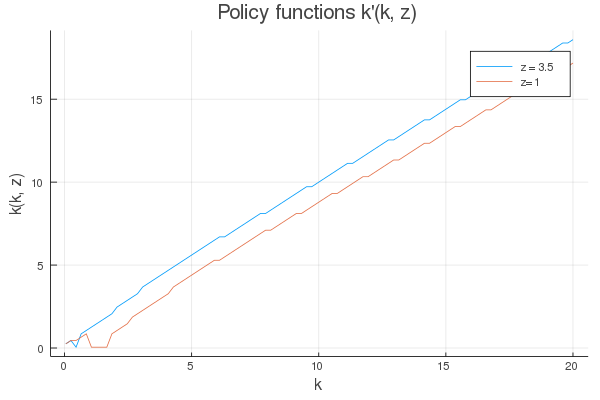
\includegraphics[width=1.2\textwidth]{cap_policy_3_b.png} % first figure itself
        \caption{Capital Policy Function}
    \end{minipage}\hfill
    \begin{minipage}{0.45\textwidth}
        \centering
        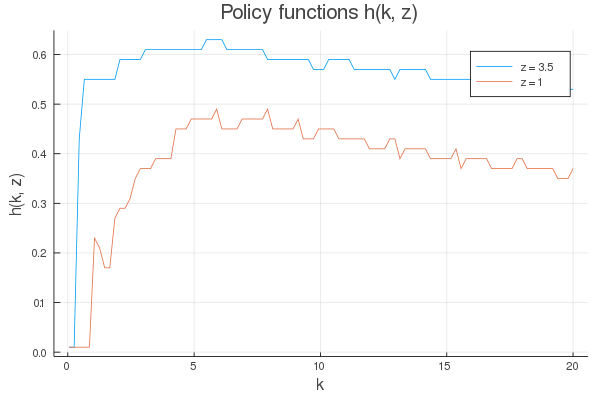
\includegraphics[width=1.2\textwidth]{lab_policy_3_b.png} % second figure itself
        \caption{Labor Policy function}
    \end{minipage}
\end{figure}


\textbf{Note:} The above VFI graphs are from a limited number of iterations and grid points and not from entire convergence since convergence was taking too much time. But the shape of policy functions are indicative of the final results.

We note that while the shape of capital policy function remains the same, the of labour policy function changes. With the separable preferences, the labour policy function is downward sloping, in the current case for low value of capital it is upward sloping. It follows the usual downward sloping graph thereafter.

%\newpage
%\bibliography{ref}

\end{document}